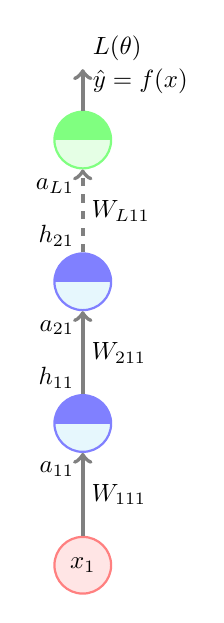
\begin{tikzpicture}[scale=0.9,transform shape]
	\tikzstyle{input_neuron}=[circle,draw=red!50,fill=red!10,thick,minimum size=8mm]
	\tikzstyle{hidden_neuron}=[circle,draw=blue!50,fill=cyan!10,thick,minimum size=8mm]
	\tikzstyle{output_neuron}=[circle,draw=green!50,fill=green!10,thick,minimum size=8mm]


	\node [input_neuron] (neuron01) at (0,0) {$x_1$};
	\node [hidden_neuron] (neuron11) at (0,2)  {};

	\begin{scope}
		\path[clip] (0,2) circle (4mm);
		\path[fill=blue!50] (-0.4,2) rectangle (0.4,2.4);
	\end{scope}


	\node [hidden_neuron] (neuron21) at (0,4)  {};


	\begin{scope}
		\path[clip] (0,4) circle (4mm);
		\path[fill=blue!50] (-0.4,4) rectangle (0.4,4.4);
	\end{scope}

	\node [output_neuron] (neuron31) at (0,6)  {};



	\begin{scope}
		\path[clip] (0,6) circle (4mm);
		\path[fill=green!50] (-0.4,6) rectangle (0.4,6.4);
	\end{scope}

	\draw[white,->] (neuron01) -- (neuron11) node[black,pos=.5,right]  {$W_{111}$} node[black,pos=0.8,left] {$a_{11}$};

	\draw[white,->] (neuron11) -- (neuron21) node[black,pos=.5,right] {$W_{211}$} node[black,pos=0.8,left] {$a_{21}$} node[black,pos=.2,left] {$h_{11}$};
	\draw[white,->] (neuron21) -- (neuron31) node[black,pos=.5,right] {$W_{L11}$} node[black,pos=0.8,left] {$a_{L1}$} node[black,pos=.2,left] {$h_{21}$};


	\draw[black!50,line width=1.5pt,->] (neuron31) -- (0,7) node[black,pos=0.7,right] {$\hat{y} = f(x)$} node[black,pos=1.5,above,right] {$\mathscr{L}(\theta)$};
	%\draw[white,->] (neuron31) -- (3,6.5) node[black,pos=1,above] {$f(x)$};
	%node[pos=1.3,above,right] {$\mathscr{L}(\theta)$};


	\foreach \from in {neuron01}
	\foreach \to in {neuron11}
	\draw [black!50,line width=1.5pt,->] (\from) -- (\to);

	\foreach \from in {neuron11}
	\foreach \to in {neuron21}
	\draw [black!50,line width=1.5pt,->] (\from) -- (\to);

	\foreach \from in {neuron21}
	\foreach \to in {neuron31}
	\draw [black!50,line width=1.5pt,dashed,->] (\from) -- (\to);


\end{tikzpicture}